\documentclass[conference]{IEEEtran}
\usepackage{times}

% numbers option provides compact numerical references in the text. 
\usepackage[numbers]{natbib}
\usepackage{multicol}
\usepackage[bookmarks=true]{hyperref}
\usepackage{graphicx,mathrsfs}


\pdfinfo{
   /Author (Homer Simpson)
   /Title  (Robots: Our new overlords)
   /CreationDate (D:20101201120000)
   /Subject (Robots)
   /Keywords (Robots;Overlords)
}

\begin{document}

% paper title
\title{Learning Simultaneous Sensory and Motor Representations- (SESEMO)}

% You will get a Paper-ID when submitting a pdf file to the conference system
\author{Berkeley Kids}

%\author{\authorblockN{Michael Shell}
%\authorblockA{School of Electrical and\\Computer Engineering\\
%Georgia Institute of Technology\\
%Atlanta, Georgia 30332--0250\\
%Email: mshell@ece.gatech.edu}
%\and
%\authorblockN{Homer Simpson}
%\authorblockA{Twentieth Century Fox\\
%Springfield, USA\\
%Email: homer@thesimpsons.com}
%\and
%\authorblockN{James Kirk\\ and Montgomery Scott}
%\authorblockA{Starfleet Academy\\
%San Francisco, California 96678-2391\\
%Telephone: (800) 555--1212\\
%Fax: (888) 555--1212}}


% avoiding spaces at the end of the author lines is not a problem with
% conference papers because we don't use \thanks or \IEEEmembership


% for over three affiliations, or if they all won't fit within the width
% of the page, use this alternative format:
% 
%\author{\authorblockN{Michael Shell\authorrefmark{1},
%Homer Simpson\authorrefmark{2},
%James Kirk\authorrefmark{3}, 
%Montgomery Scott\authorrefmark{3} and
%Eldon Tyrell\authorrefmark{4}}
%\authorblockA{\authorrefmark{1}School of Electrical and Computer Engineering\\
%Georgia Institute of Technology,
%Atlanta, Georgia 30332--0250\\ Email: mshell@ece.gatech.edu}
%\authorblockA{\authorrefmark{2}Twentieth Century Fox, Springfield, USA\\
%Email: homer@thesimpsons.com}
%\authorblockA{\authorrefmark{3}Starfleet Academy, San Francisco, California 96678-2391\\
%Telephone: (800) 555--1212, Fax: (888) 555--1212}
%\authorblockA{\authorrefmark{4}Tyrell Inc., 123 Replicant Street, Los Angeles, California 90210--4321}}


\maketitle

%\begin{abstract}
%\end{abstract}

\IEEEpeerreviewmaketitle

Redundancy reduction \cite{barlow1961possible}, edge detection \cite{hubel1968receptive}  and hierarchical representations \cite{krizhevsky2012imagenet} have been the main stay for lot of work in computer vision and vision neuroscience to represent sensory data. But, these representations do not directly lend themselves to action. It has been hypothesized \cite{o2001sensorimotor} that brain probably represents sensory information in a way that helps an organism to act in the world.  

Philipona and O'Regan \cite{philipona2003there,philipona2003perception} showed that the joint manifold of sensory and action space taken together has a lower dimensionality than that obtained by simply adding the dimensions of motor and sensory spaces. An observation which explains this is that motion of an object in the world and the equal but opposite motion of the organism with the object being stationary leads to the same sensory percept. It`s the relative motion which matters. In other words, sensory and motor spaces are `compensable'. This insight is probably employed by organisms to achieve stability of percept. For example, even when we humans are moving we perceive the world to be stationary. 

In this work we consider the problem of jointly learning sensory and motor representations which would allow an agent to act in its environment. We assume that agent has no apriori knowledge of it's kinematic model nor does it have any meaningful representations of it's sensory stimulus, i.e. the agent is the state of `tabula rasa'.  

How then can we go about building a model that models the manifold of the sensory space but with knowledge of it's relationship with the motor system? 

In this work we wish to explore this problem by introducing two ideas 
\begin{itemize}
\item Learning a basis space that represent motor actions 
\item Joint estimation of both sensory and motor representations
\item Representations that are flexible
\end{itemize}


In over actuated motor systems (high degrees of Freedom) training a controls model becomes challenging. While, there are many approaches of training such a model, we are interested in a framework that can help learn the dynamics of the many control systems an agent may have for many tasks. We propose that this can be achieved when a global objective is minimized simultaneously that learns  both sensory and motor systems. An added advantage of such representations is that, once learnt, the problem is no longer solving an optimization problem but inferring coefficients on a learnt basis. This mimics biological plasticity \cite{kandel2000principles} more closely and we argue that for a robotic agent, a hierarchical control system with some low-level reflex circuits that are modulated by high level control systems that are task dependent can effect a more versatile system.

We take the specific case of percept stabilization as an example for the agent to have an invariant representation of an image (with or without objects). Through this example, we hope to motivate that a new class of models can be imagined for learning sensorimotor representations.

\section{Model}
\textbf{I} is the Image that falls on the retina (say). From this image, we learn our sensory representation \textbf{S}. From \textbf{S}, we infer our representation \textbf{$\alpha$}. We then apply a matrix transformation $\mathcal{G}$ that takes us from the sensory space to the motor actuator space. Here, we learn a motor representation \textbf{M} and the coefficients \textbf{$\beta$} are not inferred but are a transformation based on the sensory estimate. The transformation $\mathcal{F}$ lets us go from the Motor actuator space to transforming our self, so that we can compute an error estimate. 

\begin{figure}
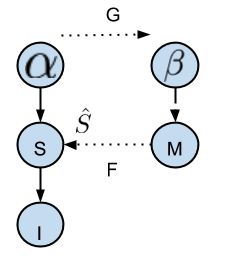
\includegraphics[scale=0.6]{sesemo1.png}
\caption{A loosely defined graphical model that describes the problem sensorimotor representations. }
\end{figure}

In our case, we define the objective to be tracking a point light source in a virtual world. We are given a camera plane and two motors that control the camera. Further, we parameterize the motor space. That is, to move the camera in the x-y plane all we have to do is apply varying powers to the two different motors. In stead of solving for the appropriate amount of power at each time step, we put forward an idea of motor representation for controlling the camera. This motor representation is a collection of tuples that specify the power to the two different motors. 

\begin{eqnarray}
\min_{S,\alpha^{t}} \| I - S\alpha^{t} \|_{2} + \lambda \| \alpha^{t} \|_{1}\\
\min_{G,M}  \| dx - (center + \mathcal{F} \beta_{t+1}^{T}M ) \|_{2} + \|G \|_{2}\\
\textit{where}\\
\beta_{t+1} = \alpha_{t} G
\end{eqnarray}


The way we go about solving the various parameters is by solving the problem in stages. The interesting idea with this model is that the sensory representation can be learnt independently as well with little loss of generality. For the rest of this work, we will not describe talking about learning the Sensory representations and focus on trying to learn the Motor basis with coefficients that are not inferred but are transformed (G) versions of inferred sensory coefficients. For our experiments we also fix our Sensory basis (S) to be a bunch of vectors that point in eight different directions that the light source may have traveled from the previous frame.

An important point to note is that our model is not completely without supervision. For the model to learn the consequences of it's motor actions we use a teacher signal (dx) that tells the system how the motor actions effect the state of the system. Another point of interest is that we begin our system with the agent not knowing the dynamics of it's control system. That is, it does not know what forward/backward/left/right are but by minimizing a global objective function it learns how to control it's motor to attain specific trajectories. 

The data in this case are 10000 samples of a point light source moving according to the following equation 
\begin{eqnarray}
r = a + b cos(k \theta),\textit{where } \theta = [ -\pi, \pi ] \\
x = r cos(\theta)\\
y = r sin(\theta)\\
\end{eqnarray}

To solve (equation 2.2) we take our current estimate of $\alpha$ and multiply it with matrix $G$ (which is either learnt or fixed as a random matrix). This is our estimate of $\beta$. We then solve for M,G using BFGS as the solver. The model learns pretty quickly and takes only a few 100 samples to converge. We then test our model on a different value of k in the above equation for about 100 samples.

The results of our experiments are summarized in the table below. Row 1 describes the experiments with learning only the Motor basis. Row 2 describes experiments with learning both the motor basis M and the sensorimotor transform G. Row 3 describes experiments with learning both the Motor basis (M) and the sensorimotor transform G but with an extra constraint on minimizing the norm of G. From our experiments, this was the best model. Systemic errors occurred during the sharp turns that we see in the data, we hypothesize that with a more sophisticated planning component in the motor planning part of the model, this can be overcome. The motor space learnt tiles the set of directions we would want the camera to move in, increasing the over completeness resulted in a more granular representation of the 3D space.

\begin{figure}
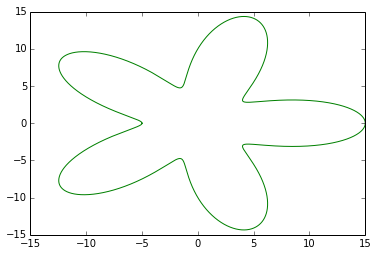
\includegraphics[scale=0.6]{train1.png}
\caption{A loosely defined graphical model that describes the problem sensorimotor representations. }
\end{figure}

% Requires the booktabs if the memoir class is not being used
\begin{table}[htbp]
   \centering
   %\topcaption{Table captions are better up top} % requires the topcapt package
   \begin{tabular}{@{} lcr @{}} % Column formatting, @{} suppresses leading/trailing space
      \multicolumn{2}{c}{A Comparison of Models } \\
      \textbf{Model}    & \textbf{Euclidean Error} \\
      \hline
      M      & 68.01 \\                
      M,G       &  13.95 \\
      M,$\|G\|_{2}$       & 0.58 \\
      
   \end{tabular}
   \caption{The table depicts the errors we see while learning variations of the model.}
   \label{tab:booktabs}
\end{table}

\section{Discussion}

We present preliminary work in trying to explore a model that tries to learn a motor representation to track an object based on its sensory representations. We show that a simple model can be learnt without having to learn the effects of the motor actions on the sensory space directly, which is a high dimensional, non-linear and complex space. We argue that by posing problems in this way with a global objective, we can explore various parts of the control space effectively because it is bounded by the task and the sensory representation. Similarly, the sensory representation that is learnt (not done in this work) is also directed towards action as opposed to a representation that is purely for redundancy reduction (compression) or to ask questions such as object recognition.

We note that, our model as it stands, is still nascent. Extensions of this model would be along the following lines
\begin{itemize}
\item Sensory representations are spatio-temporal filters along the lines of Cadieu and Olshausen \cite{cadieu2012learning}
\item One can then repose the problem of object tracking as minimizing motion energy. That is, we want to minimize the derivative of the phase coefficients of the model, so that a constant action can be chosen so as to stabilize the percept
\item Reposing the problem in the above way also changes the role of $\mathcal{F}$.  $\mathcal{F}$ is no longer a transformation of the self but a prediction of the percept from the motor system i.e. $\mathcal{P}(\alpha^{t+1} | \beta^{t+1})$. We then compare this estimate with $\mathcal{P}(\alpha^{t+1} | \alpha^{t}, S)$.
\item A model such as the above is a loopy graphical model which can be quite challenging to train. But, a model such as the above is also biologically plausible with sensory systems making motor predictions and vice-versa. Further, a representational motor space can be more efficient to work with once trained.
\end{itemize}

\section{ Acknowledgments} 

Discussions with Jitendra Malik and Tony Bell motivated a lot of this work as well. Special thanks to Pavan Ramkumar, Northwestern University for helping clarify a lot of ideas through discussions. Special thanks to Bruno Olshausen for urging us to think about sensorimotor representations. We would also like to thank our respective funding agencies - Fulbright Scholar Program. NGA. NIH. UC Berkeley.

All the code for this project can be found on our github\footnote{github.com/rctn/sesemo} link.


\bibliography{cs287_final}
\bibliographystyle{plainnat}

\end{document}


